\begin{frame}
	\frametitle{Definição}
	\par "Uma série de passos \textbf{finitos} e \textbf{bem definidos} que resolvem um determinado problema".
	\par Sendo assim, um algoritmo deve permitir uma \textbf{entrada} que, consequentemente, gerará uma \textbf{saída}.
	\begin{figure}
		\centering
		\includegraphics[width=0.3\linewidth]{images/oQueSaoAlgoritmos}
		\caption{Algoritmo}
		\label{fig:oquesaoalgoritmos}
	\end{figure}
	
\end{frame}

\begin{frame}
	\frametitle{Exemplos}
	\par "Ande".
	\par "Transações".
	\par "Faça um bolo".
	\par "Resolva uma equação".
\end{frame}

\begin{frame}
	\frametitle{Testando o algoritmo}
	\begin{itemize}
		\item Experimentação.
		\item Análise assintótica.
	\end{itemize}
	\par O foco é no tempo de execução e consumo de memória.
\end{frame}

\begin{frame}
	\frametitle{Testando o algoritmo}
	\framesubtitle{Tempo de execução}
	\par O tempo de execução pode variar segundo:
	\begin{itemize}
		\item A natureza do problema: Tamanho da entrada, formato da entrada, complexidade.
		\item Hardware: Tipo e quantidade de processadores, discos, etc.
		\item Software: Kernel, escalonamento de processos, prioridades de processo.
	\end{itemize}
\end{frame}

\begin{frame}
	\frametitle{Testando o algoritmo}
	\framesubtitle{Experimentação}
	\par Na experimentação geralmente se mede o tempo de execução variando-se, se possível, a quantidade de núcleos, processos, memória e/ou diferentes formas de escalonamento.\newline
	
	\par Um cuidado que deve ser tomado nesse tipo de teste é que algum caso particular pode não ser detectado, resultando assim em comportamentos inesperados para certas entradas, portanto, em alguns casos a experimentação sozinha não é suficiente.\newline
	
	\par Exemplo: Para uma entrada 1500 elementos um algoritmo \textbf{A} executa melhor que um algoritmo \textbf{B}, por isso, você deseja usa-lo. Será que essa opção foi a melhor, porque? 
\end{frame}

\begin{frame}
	\frametitle{Testando o algoritmo}
	\framesubtitle{Experimentação}
	\begin{figure}
		\centering
		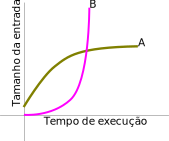
\includegraphics[width=0.5\linewidth]{images/graficoAlgoAeB}
		\caption{Comparação entre algoritmos}
		\label{fig:graficoalgoaeb}
	\end{figure}
	 
\end{frame}



